\uuid{4GOF}
\exo7id{5532}
\titre{exo7 5532}
\auteur{rouget}
\organisation{exo7}
\datecreate{2010-07-15}
\isIndication{false}
\isCorrection{true}
\chapitre{Courbes planes}
\sousChapitre{Coordonnées polaires}
\module{Géométrie}
\niveau{L2}
\difficulte{}

\contenu{
\texte{
Soit la courbe d'équation polaire $r=a(1+\cos\theta)$, $a>0$.
}
\begin{enumerate}
    \item \question{Construire la courbe.}
\reponse{\textbf{Domaine d'étude.} La fonction $r$ est $2\pi$-périodique et paire. Donc on étudie et on construit la courbe quand $\theta$ décrit $[0,\pi]$ et on obtient la courbe complète par réflexion d'axe $(Ox)$.
\textbf{Variations et signe de $r$.} La fonction $r$ est strictement décroissante sur $[0,\pi]$, strictement positive sur $]0,\pi]$ et s'annule en $\pi$.
\textbf{Etude pour $\theta=\pi$.} La tangente en $M(\pi)=O$ est la droite passant par $O$ d'angle polaire $\pi$ c'est-à-dire l'axe $(Ox)$. Par symétrie par rapport à $(Ox)$, le point $M(\pi)$ est un point de rebroussement de première espèce.

$$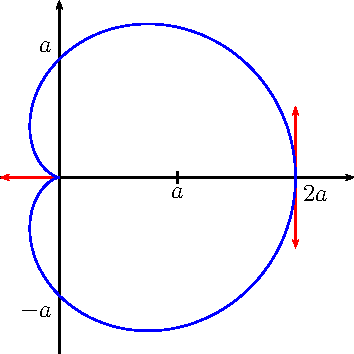
\includegraphics{../images/pdf/4GOF-1.pdf}$$}
    \item \question{Longueur et développée.}
\reponse{Soient $\theta\in[-\pi,\pi]$ puis $M=O+a(1+\cos\theta)\overrightarrow{u}_{\theta}$ le point de $\mathcal{C}$ de paramètre $\theta$. 

\begin{align*}\ensuremath
\overrightarrow{\frac{dM}{d\theta}}&=-a\sin\theta\overrightarrow{u}_{\theta}+a(1+\cos\theta)\overrightarrow{v}_{\theta}=2a\cos\left(\frac{\theta}{2}\right)\left(-\sin\left(\frac{\theta}{2}\right)\overrightarrow{u}_{\theta}+\cos\left(\frac{\theta}{2}\right)\overrightarrow{v}_{\theta}\right)\\
 &=2a\cos\left(\frac{\theta}{2}\right)\left(\cos\left(\frac{\theta}{2}+\frac{\pi}{2}\right)\overrightarrow{u}_{\theta}+\sin\left(\frac{\theta}{2}+\frac{\pi}{2}\right)\overrightarrow{v}_{\theta}\right)=2a\cos\left(\frac{\theta}{2}\right)\overrightarrow{u}_{\frac{3\theta}{2}+\frac{\pi}{2}}.
\end{align*}
\textbf{Longueur $\ell$ de la cardioïde.} On a $\left\|\overrightarrow{\frac{dM}{d\theta}}\right\|=\left|2a\cos\left(\frac{\theta}{2}\right)\right|=2a\cos\left(\frac{\theta}{2}\right)$ (pour $\theta\in[-\pi,\pi]$) et donc

\begin{center}
$\ell=\int_{-\pi}^{\pi}\left\|\overrightarrow{\frac{dM}{d\theta}}\right\|d\theta=2a\int_{-\pi}^{\pi}\cos(\theta/2)\;d\theta=4a\left[\sin(\theta/2)\right]_{-\pi}^\pi=8a$.
\end{center}

\begin{center}
\shadowbox{
La cardioïde d'équation polaire $r=a(1+\cos\theta)$, $a>0$, a pour longueur $8a$.
}
\end{center}
\textbf{Développée.} Le point $M(\theta)$ est régulier si et seulement si $\theta\neq\pm\pi$. Dans ce cas, 

\begin{center}
$\frac{ds}{d\theta}=\left\|\overrightarrow{\frac{dM}{d\theta}}\right\|=2a\cos\left(\frac{\theta}{2}\right)$ et aussi $\overrightarrow{\tau}(\theta)=\overrightarrow{u}_{\frac{3\theta}{2}+\frac{\pi}{2}}$
\end{center}

En notant $\alpha(\theta)$ une mesure de l'angle $\left(\overrightarrow{i},\overrightarrow{\tau}(\theta)\right)$, on peut prendre $\alpha(\theta)=\frac{3\theta}{2}+\frac{\pi}{2}$. En notant $R(\theta)$ le rayon de courbure au point $M(\theta)$,

\begin{center}
$R(\theta)=\frac{ds}{d\alpha}=\frac{ds/d\theta}{d\alpha/d\theta}=\frac{4}{3}a\cos\left(\frac{\theta}{2}\right)$.
\end{center}
Ensuite, $\overrightarrow{n}(\theta)=r_{\pi/2}\left(\overrightarrow{\tau}(\theta)\right)=-\overrightarrow{u}_{3\theta/2}$ et donc, en notant $\Omega(\theta)$ le centre de courbure au point $M(\theta)$,

\begin{align*}\ensuremath
\Omega(\theta)&=M(\theta)+R(\theta)\overrightarrow{n}(\theta)\\
 &=O+a(1+\cos\theta)\overrightarrow{u}_\theta-\frac{4}{3}a\cos\left(\frac{\theta}{2}\right)\overrightarrow{u}_{3\theta/2}\\
  &=O+a(1+\cos\theta)\left(\cos(\theta)\overrightarrow{i}+\sin(\theta)\overrightarrow{j}\right)-\frac{4}{3}a\left(\cos\left(\frac{\theta}{2}\right)\cos\left(\frac{3\theta}{2}\right)\overrightarrow{i}+\cos\left(\frac{\theta}{2}\right)\sin\left(\frac{3\theta}{2}\right)\overrightarrow{j}\right)\\
  &=O+a\left[\left(\cos(\theta)+\cos^2(\theta)-\frac{2}{3}(\cos(\theta)+\cos(2\theta))\right)\overrightarrow{i}+\left(\sin(\theta)+\sin(\theta)\cos(\theta)-\frac{2}{3}(\sin(\theta)+\sin(2\theta))\right)\overrightarrow{j}\right]\\
    &=O+a\left[\left(\frac{2}{3}+\frac{1}{3}\cos(\theta)-\frac{1}{3}\cos^2(\theta)\right)\overrightarrow{i}+\left(\frac{1}{3}\sin(\theta)-\frac{1}{3}\sin(\theta)\cos(\theta)\right)\overrightarrow{j}\right]\\
    &=O+\frac{2a}{3}\overrightarrow{i}+\frac{a}{3}(1-\cos\theta)\overrightarrow{u}_\theta
\end{align*}
Notons $\Gamma$ la développée cherchée. On a $\Gamma=t\circ h(\mathcal{C}_1)$ où $t$ est la translation de vecteur $\frac{2a}{3}\overrightarrow{i}$, $h$ est l'homothétie de centre $O$ et de rapport $\frac{1}{3}$ et $\mathcal{C}_1$ la courbe d'équation polaire $r=a(1-\cos\theta)$.
Maintenant, en notant $r$ la fonction $\theta\mapsto a(1+\cos\theta)$ et $r_1$ la fonction $\theta\mapsto a(1-\cos\theta)$, 

\begin{center}
$[r_1(\theta+\pi),\theta+\pi)]=[a(1+\cos\theta),\theta+\pi]=s_O([r(\theta),\theta)])$.
\end{center}
La courbe $\mathcal{C}_1$ est donc la symétrique par rapport à $O$ de la courbe $\mathcal{C}$. En résumé, la développée de $\mathcal{C}$ est l'image de $\mathcal{C}$ par la transformation $t\circ h\circ s_O$ : c'est encore une cardioïde.

$$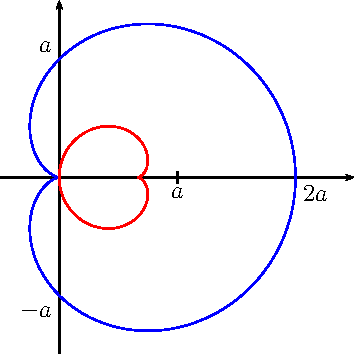
\includegraphics{../images/pdf/4GOF-2.pdf}$$}
\end{enumerate}
}
